\chapter{Introduction}
Endodontic treatment, also known as root canal treatment and nerve extraction, is performed to cure an infected tooth. The procedure of endodontic treatment is divided into three parts - Opening, Cleaning, and Filling shown in  Figure \ref{fig:endo-procedure}.
\begin{figure}[htbp]
\begin{center}
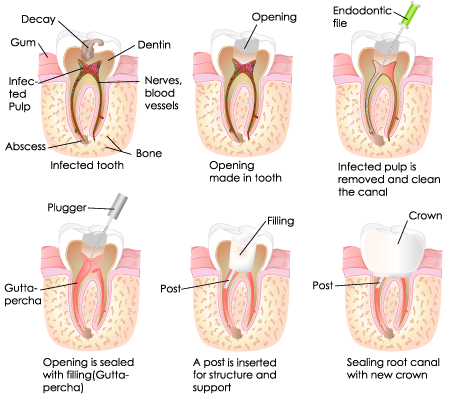
\includegraphics[width=0.8\linewidth]{Images/endo-procedure.png}
\caption{
The endodontic therapy steps
}\label{fig:endo-procedure}
\end{center}
\end{figure}
\newpage
An infected tooth results from periodontal disease, attrition, trauma, or decay. Once the dental pulp is infected, it causes an irreversible inflammation and let patients confront a root canal treatment. Figure \ref{fig:endo-procedure} shows an infected tooth and its dental pulp, which consisted of blood vessels, nerves, connective tissues, and lymphatics. In the "Opening" step, an experienced dentist drills the crown of infected tooth to remove the dentin and expose the infected pulp inside the canal to the air. Next, in the "Cleaning" step the dentist uses an endodontic file which is a flexible reamer to remove the infected pulp. Then, in the "Filling" step the dentist uses a dental plugger to fill the empty root canal with Gutta-percha which is a plastic substance. "Filling" can prevent cross infection between root canals because the cured teeth remains many invisible and inaccessible pulp tissue. Finally the dentist seals root canal with new crown to protect cured root canal. 
\par
"Cleaning" is of paramount importance in a whole treatment because untreated cleaning will result in pulp necrosis, apical abscess, periodontal ligament inflammation, or even cellulitis. If there are many remained infected pulp after root canal treatment, the surgery should be operated on again.
\section{Motivation}
The performance of the endodontic treatment depends on the dentist's own long-term experience. A qualified dentist can operate the endodontic treatment and accumulate their experience to increase the success rate. With many experiences, dentists can acquire an endodontist license. According to statistics from the Ministry of Health and Welfare, R.O.C. (Taiwan), the number of dentists in Taiwan is $15,178$. However, according to The Academy of Endodontology, R.O.C. (Taiwan), there are only $238$ dentists to acquire an endodontist license due to the expertise of endodontics. Besides, Root canal treatment is tedious and time-consuming due to complicated conditions of each tooth, a patient who suffered from an infected tooth spends much time see a dentist It takes at least two to three rounds, even spends more than two months in the worst case. 
\par
Therefore, our team looks forward to designing a robot-assisted system to finish the root canal treatment. The definition of robot-assisted system in the present thesis refers to be a dental assistant. With the system, we wish it can increase the success rate for dentists and provide patients a safe surgery.

\section{Previous Work and Problem Definition}
Use present tense.
(Previous work: briefly mention the existing dental robots)
\par\noindent
(Problem definition:
1.	Assist dentists to operate RCT and focus on cleaning procedure
2.	Root canal cannot be visually observed and is too small to clean well
3.	Risk of file breakage)		
\par\noindent
Instruments fracture and perforation are two problems that commonly occur during the therapy. Removal of broken files is both technically difficult and therefore it is important to reduce the probability of fracture. In addition, root canal treatment also requires repeatedly drilling in order to clean the canal thoroughly.  This repetitive action of root canal treatment is tedious and time-consuming. Therefore, we designed an automatic endodontic robot to improve the time-efficiency and to reduce the occurrence of instrument fracture in endodontic surgery.
The root canal cleaning is a big challenge in and of itself
There is one robotic system that is designed to perform endodontic therapy. In Intelligent Micro Robot Development for Minimum Invasive Endodontic Treatment [3] , they proposed a micro robot performing root canal treatment with the assistance of 3D computer model system. It is designed to accomplish endodontic therapy with path planned according to the 3D model. However, the problem of instruments fracture still remains. 
In this paper, a torque monitoring method is proposed. The main causes of fractured files are torsional fracture and flexural fatigue, account for 55.7\% and 44.3\% separately [5]. Therefore, we use current feedback to keep track of the torque which the file is bearing during the endodontic treatment. This torque monitoring system is implemented on an endodontic robot prototype we built. We primarily focus on the cleaning and shaping step since it’s the key step to a successful root canal treatment. With the robot prototype and torque monitoring system, the possibility of instrument fracture can be reduced. Besides, the repetitive action during the drilling step can be performed by the robot.			
\section{The Proposed Method}
(Solutions: (be consistent with problem definition)
1.	Build a robot-assisted system and enable it to drill
2.	Force-guided alignment 
3.	Control the file rotation speed
B.	Prospect:
\par\noindent
(Prospect: Move to the infected teeth$\longrightarrow $Root canal searching$\longrightarrow $Repetitive drilling$\longrightarrow $Apex Detection)						
\section{Main Contributions of the Thesis}
\begin{enumerate}
	\item	Integrate a 6-DoF robotic manipulator with 6-DoF F/T sensor for performing endodontic treatment.
	\item	Develop a framework for robot alignment regarding the position and orientation of root canal. 
	\item	Protect the endodontic file from fracturing by controlling file rotation speed.
\end{enumerate}
\section{Organization of the Thesis}